%%%%%%%%%%%%%%%%%%%%%%%%%%%%%%%%%%%%%%%%%
% Wenneker Assignment
% LaTeX Template
% Version 2.0 (12/1/2019)
%
% This template originates from:
% http://www.LaTeXTemplates.com
%
% Authors:
% Vel (vel@LaTeXTemplates.com)
% Frits Wenneker
%
% License:
% CC BY-NC-SA 3.0 (http://creativecommons.org/licenses/by-nc-sa/3.0/)
% 
%%%%%%%%%%%%%%%%%%%%%%%%%%%%%%%%%%%%%%%%%

%----------------------------------------------------------------------------------------
%	PACKAGES AND OTHER DOCUMENT CONFIGURATIONS
%----------------------------------------------------------------------------------------

\documentclass[11pt]{scrartcl} % Font size

%%%%%%%%%%%%%%%%%%%%%%%%%%%%%%%%%%%%%%%%%
% Wenneker Assignment
% Structure Specification File
% Version 2.0 (12/1/2019)
%
% This template originates from:
% http://www.LaTeXTemplates.com
%
% Authors:
% Vel (vel@LaTeXTemplates.com)
% Frits Wenneker
%
% License:
% CC BY-NC-SA 3.0 (http://creativecommons.org/licenses/by-nc-sa/3.0/)
% 
%%%%%%%%%%%%%%%%%%%%%%%%%%%%%%%%%%%%%%%%%

%----------------------------------------------------------------------------------------
%	PACKAGES AND OTHER DOCUMENT CONFIGURATIONS
%----------------------------------------------------------------------------------------

\usepackage{amsmath, amsfonts, amsthm} % Math packages

\usepackage{listings} % Code listings, with syntax highlighting

\usepackage[english]{babel} % English language hyphenation

\usepackage{graphicx} % Required for inserting images
\graphicspath{{Figures/}{./}} % Specifies where to look for included images (trailing slash required)

\usepackage{booktabs} % Required for better horizontal rules in tables

\numberwithin{equation}{section} % Number equations within sections (i.e. 1.1, 1.2, 2.1, 2.2 instead of 1, 2, 3, 4)
\numberwithin{figure}{section} % Number figures within sections (i.e. 1.1, 1.2, 2.1, 2.2 instead of 1, 2, 3, 4)
\numberwithin{table}{section} % Number tables within sections (i.e. 1.1, 1.2, 2.1, 2.2 instead of 1, 2, 3, 4)

\setlength\parindent{0pt} % Removes all indentation from paragraphs

\usepackage{enumitem} % Required for list customisation
\setlist{noitemsep} % No spacing between list items

%----------------------------------------------------------------------------------------
%	DOCUMENT MARGINS
%----------------------------------------------------------------------------------------

\usepackage{geometry} % Required for adjusting page dimensions and margins

\geometry{
	paper=a4paper, % Paper size, change to letterpaper for US letter size
	top=2cm, % Top margin
	bottom=2cm, % Bottom margin
	left=2cm, % Left margin
	right=2cm, % Right margin
	headheight=0.75cm, % Header height
	footskip=1.5cm, % Space from the bottom margin to the baseline of the footer
	headsep=0.75cm, % Space from the top margin to the baseline of the header
	%showframe, % Uncomment to show how the type block is set on the page
}

%----------------------------------------------------------------------------------------
%	FONTS
%----------------------------------------------------------------------------------------

\usepackage[utf8]{inputenc} % Required for inputting international characters
\usepackage[T1]{fontenc} % Use 8-bit encoding

\usepackage{fourier} % Use the Adobe Utopia font for the document

%----------------------------------------------------------------------------------------
%	SECTION TITLES
%----------------------------------------------------------------------------------------

\usepackage{sectsty} % Allows customising section commands

\sectionfont{\vspace{6pt}\centering\normalfont\scshape} % \section{} styling
\subsectionfont{\normalfont\bfseries} % \subsection{} styling
\subsubsectionfont{\normalfont\itshape} % \subsubsection{} styling
\paragraphfont{\normalfont\scshape} % \paragraph{} styling

%----------------------------------------------------------------------------------------
%	HEADERS AND FOOTERS
%----------------------------------------------------------------------------------------

\usepackage{scrlayer-scrpage} % Required for customising headers and footers

\ohead*{} % Right header
\ihead*{} % Left header
\chead*{} % Centre header

\ofoot*{} % Right footer
\ifoot*{} % Left footer
\cfoot*{\pagemark} % Centre footer
 % Include the file specifying the document structure and custom commands

%----------------------------------------------------------------------------------------
%	TITLE SECTION
%----------------------------------------------------------------------------------------
\usepackage{float}
\title{	
	Homework 3
}
\usepackage{xcolor}
\lstset{
    columns=fixed,       
    numbers=left,                                        % 在左侧显示行号
    frame=none,                                          % 不显示背景边框
    backgroundcolor=\color[RGB]{245,245,244},            % 设定背景颜色
    keywordstyle=\color[RGB]{40,40,255},                 % 设定关键字颜色
    numberstyle=\footnotesize\color{darkgray},           % 设定行号格式
    commentstyle=\it\color[RGB]{0,96,96},                % 设置代码注释的格式
    stringstyle=\rmfamily\slshape\color[RGB]{128,0,0},   % 设置字符串格式
    showstringspaces=false,                              % 不显示字符串中的空格
    language=c++,                                        % 设置语言
}
\author{Yuan Jiahao 2019010070} % Your name

\date{\normalsize\today} % Today's date (\today) or a custom date

\begin{document}

\maketitle % Print the title

%----------------------------------------------------------------------------------------
%	FIGURE EXAMPLE
%----------------------------------------------------------------------------------------

\section{Todo}
Multiply a square matrix A of size m $\times$ m and a tall-and-skinny matrix B of size m $\times$ n
(m should be much larger than n) to get C = AB, and run the given basic code of sparse
matrix-multiple vector multiplication (SpMM) using the CSR format for A. Try to compare the
performance difference of ten different codes.

Verify the correctness of the results, test performance (note that cudaDeviceSynchronize()
should be called before timing function, and a kernel call should run 200 times, and the average
execution time should be recorded), and write a performance comparison in the report;
\section{Hardware Environment of the Machine }
The machine's CPU is Intel Core i3-10100F ,3.2GHz with 4 cores and 8 threads.The memory is 16GB,the GPU is two NVIDIA GTX-1650 crossfire,and the system is Ubuntu 20.04.

All the following codes are complied in O3 optimization and nvcc option is -gencode$=$arch$=$compute\_61, code$=$compute\_61.
\section{Analysis}
The test code will generate a CSR version matrix and convert it into normal matrix,with value 1,in each situation.So the ten types of code will be tested in the same condition with the same to test data.
\section{Result}
\subsection{Heatmap}
To have a comprehensive overview,I put the ten heatmap together here,and then we will get into some interesting conclusion.All the data's unit is GFlops,thus the data gets larger,the performance gets better.
\begin{figure}[H]
    \centering
    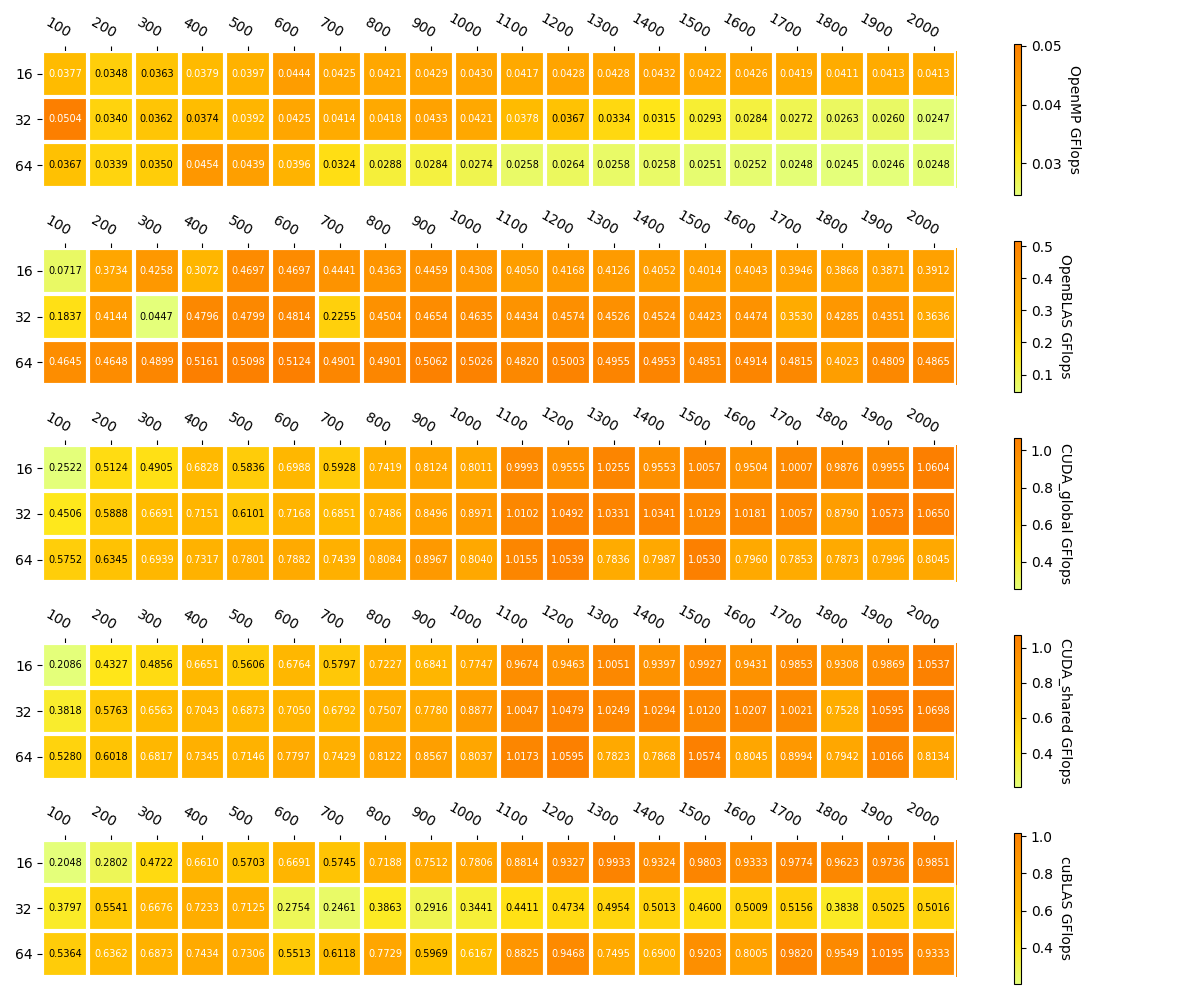
\includegraphics[width=0.9\textwidth]{Figure_1.png}
    \label{}
\end{figure}
\begin{figure}[H]
    \centering
    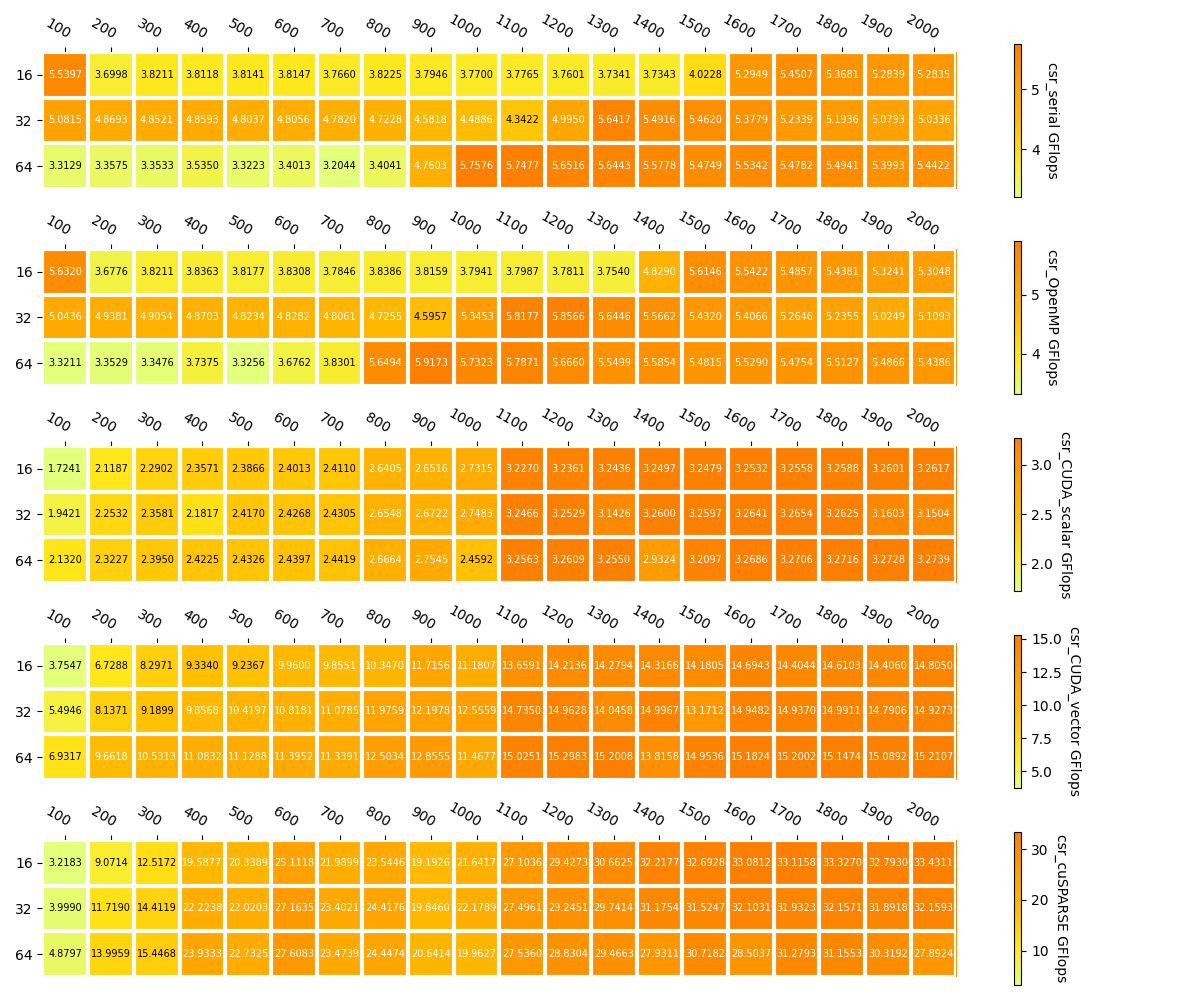
\includegraphics[width=0.9\textwidth]{Figure_2.png}
    \label{}
\end{figure}
\subsection{The comparison of performance between normal GEMM with SpMM}
Due to the matrix is sparse,the normal GEMM made a lot of unnecessary computation.Thus,all the SpMM codes performs much better than the normal GEMM codes.You see,the best normal GEMM code performance at cuBLAS is about 1 GFlops,but the best SpMM code performance could reach 33 GFlops.
\subsection{The comparison of performance between different matrix size}
Common sense is that the performance will be better when the matrix size is larger.However,it might due to the weird shape of right vector,most normal GEMM codes (except cuBLAS) perform best when matrix B size is m*32 rather than m*64,but it doesn't fit the SpMM codes,most SpMM codes performs better as the size of matrix get larger.

Anyway,in general,the performance is better as the matrix size get larger.
\subsection{More insight into the SpMM codes}
Since we have discussed the normal GEMM a lot before,thus maybe it's time to focus on the SpMM codes more.

First,we will find the serial and openMP version performs very similar,even the performance distribution between different size of matrix,both of them performs best when the m is 1200 and the width is 64.Anyway it's better than the normal GEMM codes.

What's surprised is that csr CUDA scalar version performs even worse than the serial version,but the trend is normal that the performance goes better as the matrix gets larger,without a peak.

Finally,the vector and cuSPARSE version performs very well.They reaches their peak performance at 15 GFlops and 30 GFlops respectively.
\end{document}
